\documentclass{beamer}
\usetheme{Boadilla}

\usepackage{graphicx}
\usepackage[outdir=./out/]{epstopdf}
\graphicspath{ {./images/} {../images/} }
\usepackage{subcaption}

\usepackage{amsmath}
\usepackage{mathtools}
\usepackage{amsfonts}

% This declares \abs and \norm commands
\DeclarePairedDelimiter\abs{\lvert}{\rvert}%
\DeclarePairedDelimiter\norm{\lVert}{\rVert}%

% Swap the definition of \abs* and \norm*, so that \abs
% and \norm resizes the size of the brackets, and the 
% starred version does not.
\makeatletter
\let\oldabs\abs
\def\abs{\@ifstar{\oldabs}{\oldabs*}}
%
\let\oldnorm\norm
\def\norm{\@ifstar{\oldnorm}{\oldnorm*}}
\makeatother

\AtBeginSection[]{
    \begin{frame}
    \vfill
    \centering
    \begin{beamercolorbox}[sep=8pt,center,shadow=true,rounded=true]{title}
      \usebeamerfont{title}\insertsectionhead\par%
    \end{beamercolorbox}
    \vfill
    \end{frame}
}

\title{Algorithm Engineering for Cluster Editing}
\author{Sebastian Paarmann}
%\institute{Institute for Something - TUHH} % TODO
\date{\today}

\begin{document}

\begin{frame}
	\titlepage
\end{frame}

%\begin{frame}
%	\frametitle{Outline}
%	\tableofcontents
%\end{frame}

\section{Introduction}

\begin{frame}
	\frametitle{Cluster Graphs}
	\begin{itemize}
		\item $G$ \emph{Cluster Graph} $:\Leftrightarrow$ all components of $G$ are cliques
	\end{itemize}

	\begin{figure}[h]
		\centering
		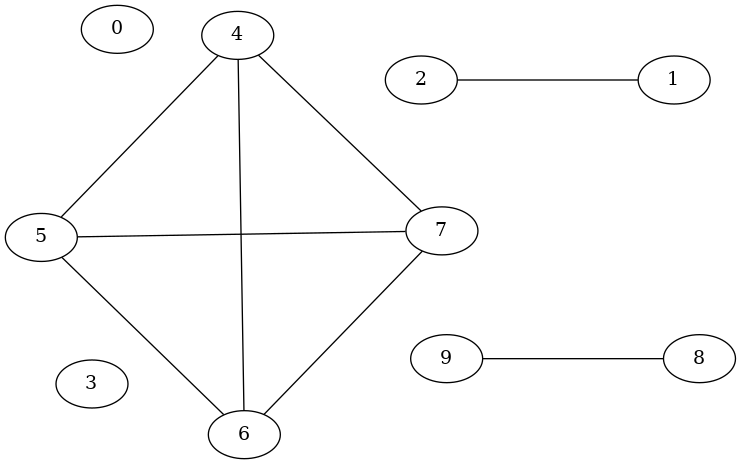
\includegraphics[width=0.7\linewidth]{exact001-output}

		\caption{A cluster graph}
	\end{figure}
\end{frame}

\begin{frame}
	\frametitle{Cluster Editing}

	\begin{itemize}
		\item Turn an input graph into a cluster graph, by inserting and deleting edges
	\end{itemize}

	\pause

	\begin{figure}[h]
		\centering
		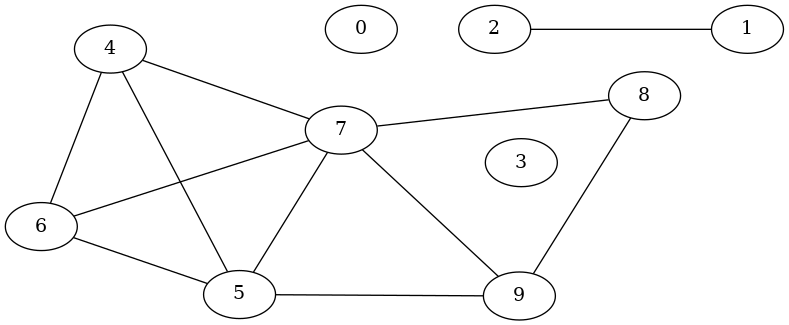
\includegraphics[width=0.5\linewidth]{exact001-input}
	\end{figure}

	\pause

	\centering
	to

	\begin{figure}[h]
		\centering
		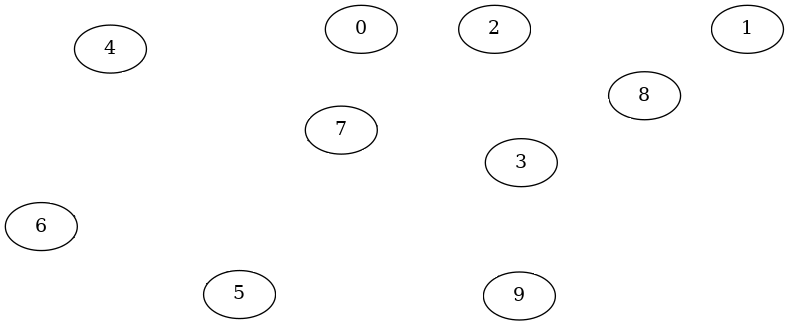
\includegraphics[width=0.5\linewidth]{exact001-no-edges}
	\end{figure}

	\centering
	?
\end{frame}

\begin{frame}
	\frametitle{Cluster Editing}
	\begin{itemize}
		\item More interesting: Turn $G$ into a cluster graph by doing as few edits as possible
		\only<3->{
			\item Motivation: bioinformatics (gene sequencing, transcriptomics, and more), machine learning
			\item In our case: ``Parameterized Algorithms and Computational Experiments'' (PACE) Challenge
			\begin{itemize}
				\item Competition to develop fast and practical solvers for the given problem (PACE
					2021: Cluster Editing)
			\end{itemize}
		}
	\end{itemize}

	\only<2>{
		\begin{figure}[h]
			\centering
			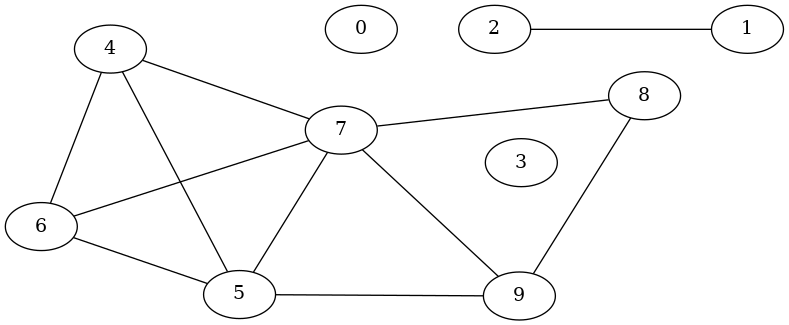
\includegraphics[width=0.49\linewidth]{exact001-input}
		\end{figure}

		\centering
		to

		\begin{figure}[h]
			\centering
			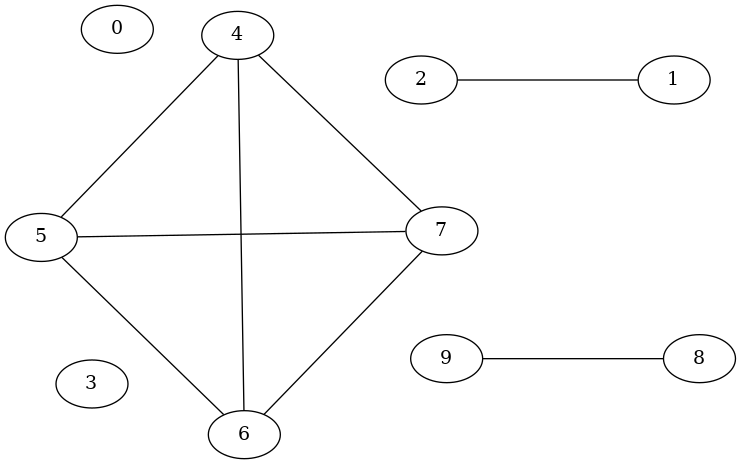
\includegraphics[width=0.49\linewidth]{exact001-output}
		\end{figure}
	}
\end{frame}

\begin{frame}
	\frametitle{Cluster Editing (Optimization Problem)}
	\begin{itemize}
		\item Input: Graph $G = (V, E)$
		\item Output: $F \subseteq \binom{V}{2}$ such that $(V, E \Delta F)$ cluster graph and
			$\abs{F}$ minimal
	\end{itemize}
\end{frame}

\section{Fixed-Parameter Algorithms}

\begin{frame}
	\frametitle{Fixed-Parameter Algorithms}
	\begin{itemize}
		\item Cluster Editing is NP-complete
		\item $\Rightarrow$ Use a \emph{fixed-parameter} approach to keep complexity manageable
		\pause
		\item A problem is \emph{fixed-parameter tractable} (FPT) $:\Leftrightarrow \exists$ an
			algorithm to solve it in time $f(k) * n^c$
	\end{itemize}
\end{frame}

\begin{frame}
	\frametitle{Parameterized Cluster Editing}
	\begin{itemize}
		\item Input: $(G, k)$
		\item Output: $F \subseteq \binom{V}{2}$ such that $(V, E \Delta F)$ cluster graph and
			$\abs{F} \leq k$, if such an $F$ exists
		\item $k$ is our \emph{parameter} and limits the size of the solution
		\item To find optimal solution, execute with increasing parameter and find the lowest value
			with a solution
	\end{itemize}
\end{frame}

\begin{frame}
	\frametitle{Fixed-Parameter Algorithms}
	\begin{itemize}
		\item Two central concepts:
		\begin{enumerate}
			\item Bounded Search Tree Algorithms
			\item Data Reduction Rules
		\end{enumerate}
	\end{itemize}
\end{frame}

\begin{frame}
	\frametitle{Bounded Search Trees}
	\begin{itemize}
		\item ``Branching Algorithm''
		\item Backtracking, taking the parameter into account
		\item Split into multiple branches, taking some decision (``delete an edge'', ``insert an
			edge''); recursively call self
		\item \emph{Bounded}: Number of recursive calls in each node limited \& each decision
			reduces the parameter
	\end{itemize}
\end{frame}

\begin{frame}
	\frametitle{Conflict Triples}
	\begin{itemize}
		\item $v, u, w \in V$ \emph{conflict triple} $:\Leftrightarrow uv, uw \in E, vw \notin E$
		\item $G$ cluster graph $\Leftrightarrow \nexists $ conflict triple in $G$
	\end{itemize}

	\begin{figure}[h]
		\centering
		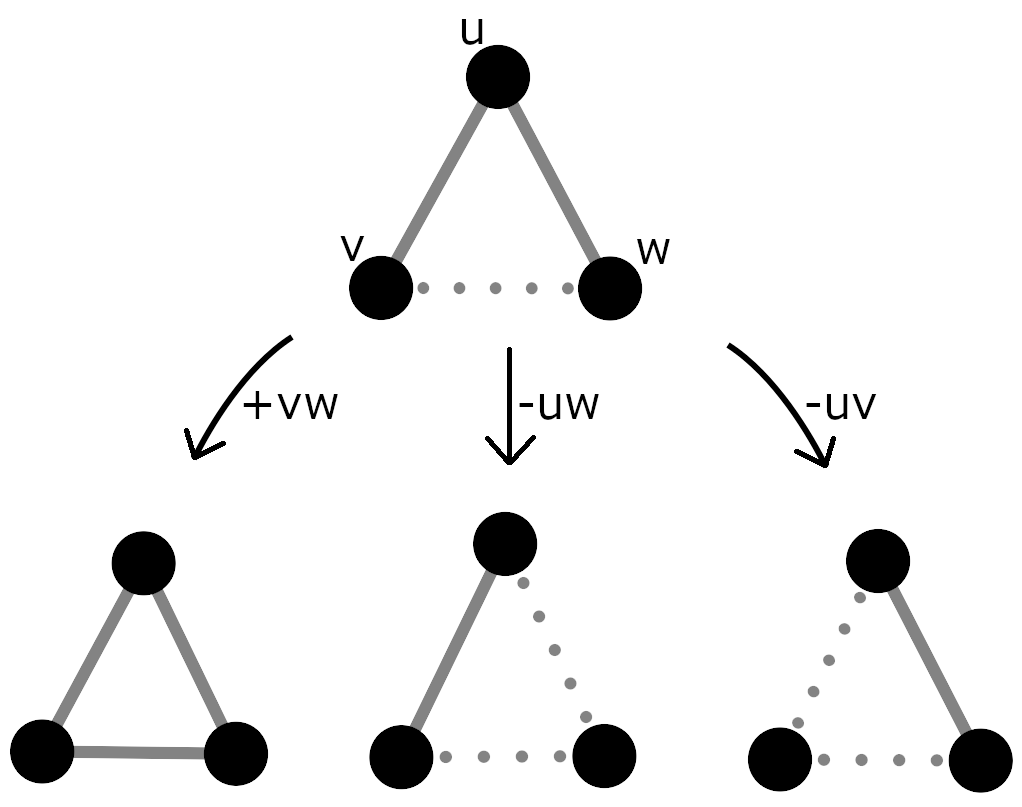
\includegraphics[scale=0.5]{conflicts}
		\caption{A conflict $v u w$ and three ways to resolve it.}
		\label{fig:conflicts}
	\end{figure}
\end{frame}

\begin{frame}
	\frametitle{Simple Branching Algorithm}
	\begin{itemize}
		\item Find a conflict triple $vuw$
			\begin{itemize}
				\item If none, return solution
			\end{itemize}
		\item Branch intro three cases:
			\begin{enumerate}
				\item Add $vw$, decrease $k$ by 1
				\item Remove $uw$, decrease $k$ by 1
				\item Remove $uv$, decrease $k$ by 1
			\end{enumerate}
	\end{itemize}

	\begin{figure}[h]
		\centering
		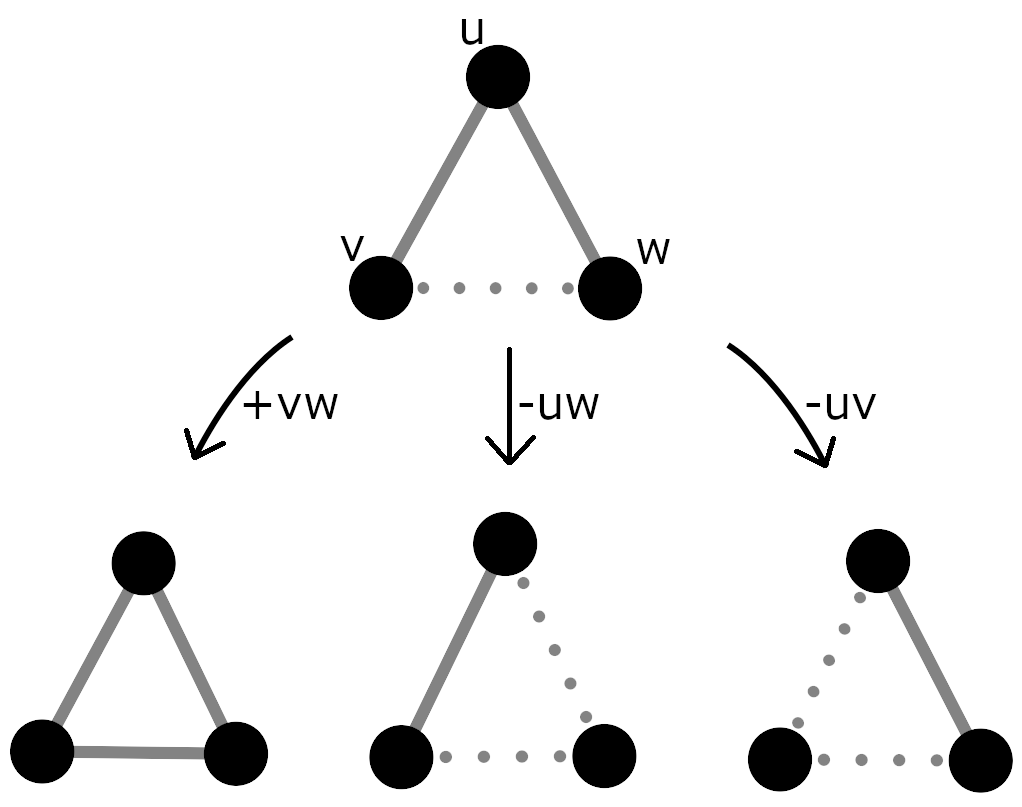
\includegraphics[scale=0.5]{conflicts}
		\caption{A conflict $v u w$ and three ways to resolve it.}
	\end{figure}
\end{frame}

\begin{frame}
	\frametitle{Weighted Cluster Editing}
	\begin{itemize}
		\item $G = (V, E), s: \binom{V}{2} \to \mathbb{Z} \cup \{-\infty, \infty\}$ \emph{weight function}
		\item $s(uv) > 0 \Leftrightarrow uv \in E$
		\item Inserting $uv$ \emph{costs} $-s(uv)$, removing $uv$ costs $s(uv)$
		\item $k$ then maximal allowed cost instead of number of edits
	\end{itemize}
\end{frame}

\begin{frame}
	\frametitle{Search Tree}
	\begin{itemize}
		\item Find conflict triple $vuw$
		\item Branch:
			\begin{enumerate}
				\item Forbid $uv$
				\item Merge $uv$
			\end{enumerate}
		\item $O(2.62^k)$ search tree
	\end{itemize}

	\vskip 20pt
	
	\begin{itemize}
		\item Böcker et al.: ``Going Weighted: Parameterized Algorithms for Cluster Editing''
	\end{itemize}
\end{frame}

\begin{frame}
	\frametitle{Merging}
	\begin{itemize}
		\item Replace $u$ and $v$ by new node $u'$
		\item $\forall w \in V: s(u'w) = s(uw) + s(vw)$
		\item Merged nodes are treated as having a permanent edge
	\end{itemize}
\end{frame}

\section{Data Reduction Rules}

\begin{frame}
	\frametitle{Reduction Rules}
	\begin{itemize}
		\item Preprocessing of input to find a smaller but equivalent instance
		\item Some reductions also applied on intermediate instances in the search tree
		\item Transform $(G, k)$ into another instance $(G', k')$
		\item Rule is \emph{correct} if $(G, k)$ has a solution $\Leftrightarrow (G', k')$ has a
			solution
		\item Rule can make the instance/graph easier, reduce the parameter, or both

		\vskip 10pt

		\item J. Guo: ``A more effective linear kernelization for cluster editing''
		\item Böcker et al.: ``A Fixed-Parameter Approach for Weighted Cluster Editing'' and ``Exact
			Algorithms for Cluster Editing: Evaluation and Experiments''
	\end{itemize}
\end{frame}

\begin{frame}
	\frametitle{Critical Cliques}
	\begin{itemize}
		\only<1>{
		\item Reduction applied in the process of making a weighted graph from the unweighted input
		\item $K \subseteq V$ \emph{critical clique} $:\Leftrightarrow K$ induced clique, vertices
			in $K$ all have same neighbors outside of $K$, $K$ is maximal under this property
		}
		\only<2>{
		\item Optimal Cluster Editings never split a critical clique up
		\item $\Rightarrow$ Merge each critical clique into one node, resulting in a reduced
			weighted graph
		}
	\end{itemize}

	\begin{figure}[h]
		\centering
		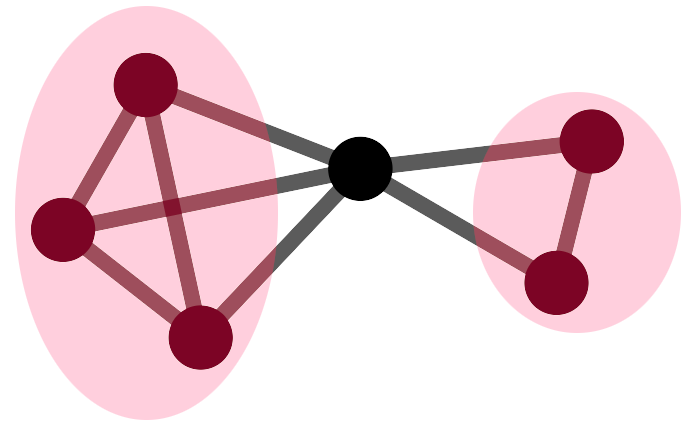
\includegraphics[width=0.7\linewidth]{crit-cliques}
	\end{figure}
\end{frame}

\begin{frame}
	\frametitle{Rules 1--3}
	\begin{figure}[h]
		\centering
		\includegraphics[width=1\textwidth]{rules1-3}
	\end{figure}
	\begin{enumerate}
		\item Forbid $uv$ with $s(uv) < 0$ if $\abs{s(uv)} \geq \sum_{w \in N(u)} s(uw)$
		\item Merge $uv$ with $s(uv) > 0$ if $s(uv) \geq \sum_{w \in V \setminus \{u, v\}} \abs{s(uw)}$
		\item Merge $uv$ with $s(uv) > 0$ if 
			\[
				s(uv) \geq \sum_{w \in N(u) \setminus \{v\}} s(uw) + \sum_{w \in N(v) \setminus \{u\}} s(vw)
			\]
	\end{enumerate}
\end{frame}

\begin{frame}
	\frametitle{Rule 4}
	\begin{itemize}
		\item Let $C \subseteq V$ and $k_C$ the min-cut value of $G[C]$
		\item Merge all vertices of $C$ if
			\[
				k_C \geq \sum_{u,v \in C, s(uv) \leq 0} \abs{s(uv)}
					+ \sum_{u \in C, v \in V \setminus C, s(uv) > 0} s(uv).
			\]
	\end{itemize}
\end{frame}

\begin{frame}
	\frametitle{Induced Costs}
	\begin{itemize}
		\item Define
			\begin{align*}
				\mathsf{icf}(uv) &= \sum_{w \in N(u) \cap N(v)} \min\{s(uw), s(vw)\} \\
				\mathsf{icp}(uv) &= \sum_{w \in (N(u) \Delta N(v)) \setminus \{u, v\}}
					\min\{\abs{s(uw)}, \abs{s(vw)}\}
			\end{align*}
		\only<1>{
		\item Where $\mathsf{icf}(uv) + \max\{0, s(uv)\} > k$: Merge $u$ and $v$
		\item Where $\mathsf{icp}(uv) + \max\{0, -s(uv)\} > k$: Forbid $uv$
		}
		%\only<2>{
		%\item Where $\mathsf{icf}(uv) + \max\{0, s(uv)\} + b(G, uv) > k$: Merge $u$ and $v$
		%\item Where $\mathsf{icp}(uv) + \max\{0, -s(uv)\} + b(G, uv) > k$: Forbid $uv$
		%}
	\end{itemize}
\end{frame}

\section{Implementation Details \& Techniques}

\begin{frame}
	\frametitle{Graph Storage}
	\begin{itemize}
		\item Symmetric square matrix of weights
		\item Also tested:
			\begin{itemize}
				\item Store only triangular matrix
				\item Hybrid weight matrix and adjacency list approaches
			\end{itemize}
		\item Boolean mask to mark nodes as removed
		\item Weights are integer values, but stored as floats for efficient hardware handling of
			infinities
	\end{itemize}
\end{frame}

\begin{frame}
	\frametitle{Merging Vertices}
	\begin{itemize}
		\item Merging changes the size of the graph
		\item Extra boolean mask to indicate removed nodes
		\item Enables removing a node almost for free
		\item Also enables \emph{undo} of a removal
	\end{itemize}
\end{frame}

\begin{frame}
	\frametitle{Undo with Oplogs}
	\begin{itemize}
		\item In each step, algorithm branches into two cases
		\item Both branches need to start from same initial state + branching operation
		\item Avoid cloning the entire state by being able to roll changes from the first branch
			back before starting the second
		\item Implemented using a list of operations, an \emph{oplog}
	\end{itemize}
\end{frame}

\begin{frame}
	\frametitle{Conflict Tracking}
	\begin{itemize}
		\item List of conflicts in the graph useful for fast branching and calculating lower bounds
		\item Tracked using a boolean mask over triples of vertices, list of edge disjoint
			conflicts, mapping of pairs of vertices to indices into the list
		\item Allows updates for edge insertion and deletion in $O(n)$ time and quickly finding a
			conflict
		\item Also supports rollback completely
	\end{itemize}
\end{frame}

\section{Results}


\begin{frame}
	\frametitle{Results}
	\begin{figure}[h]
		\begin{subfigure}{0.49\textwidth}
			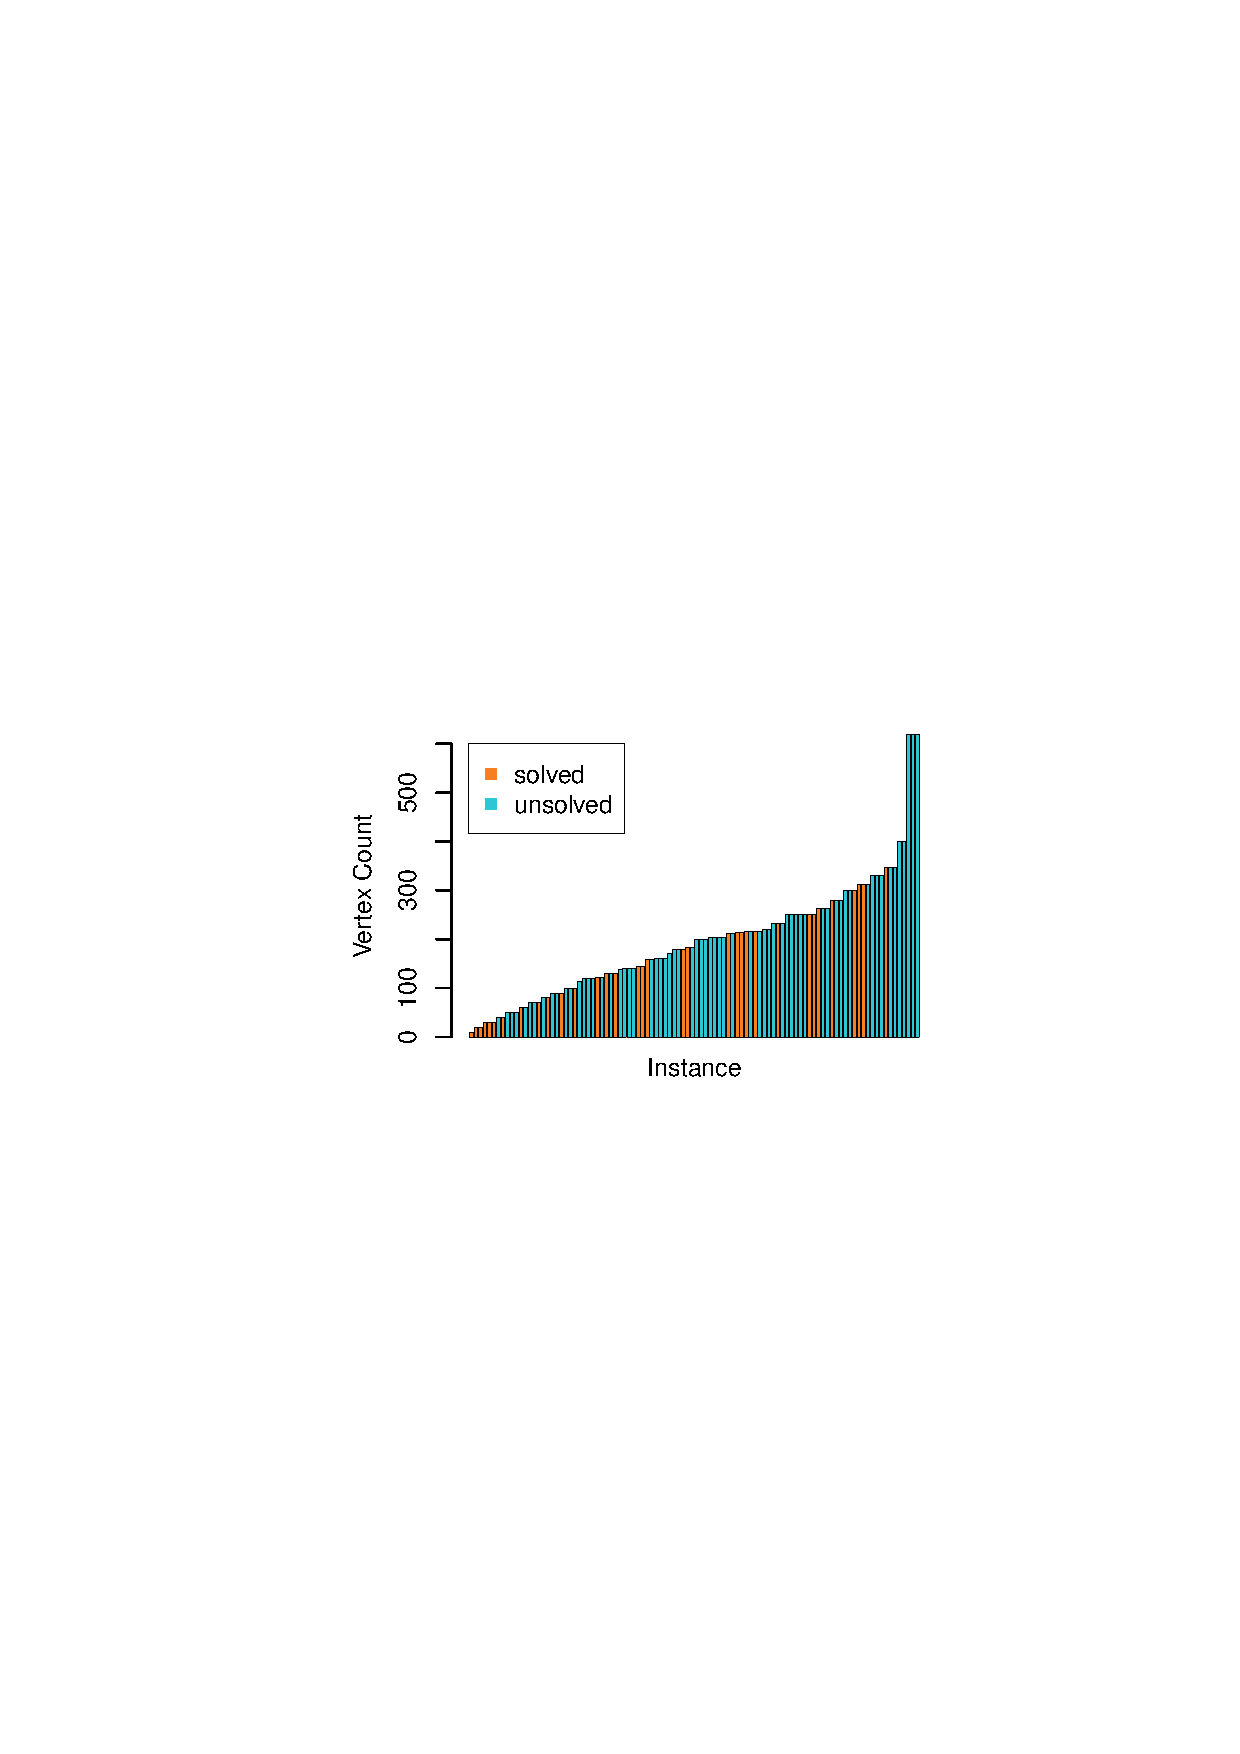
\includegraphics[width=1.0\linewidth]{instances}
			\subcaption{Instance Sizes}
		\end{subfigure}
		\begin{subfigure}{0.49\textwidth}
			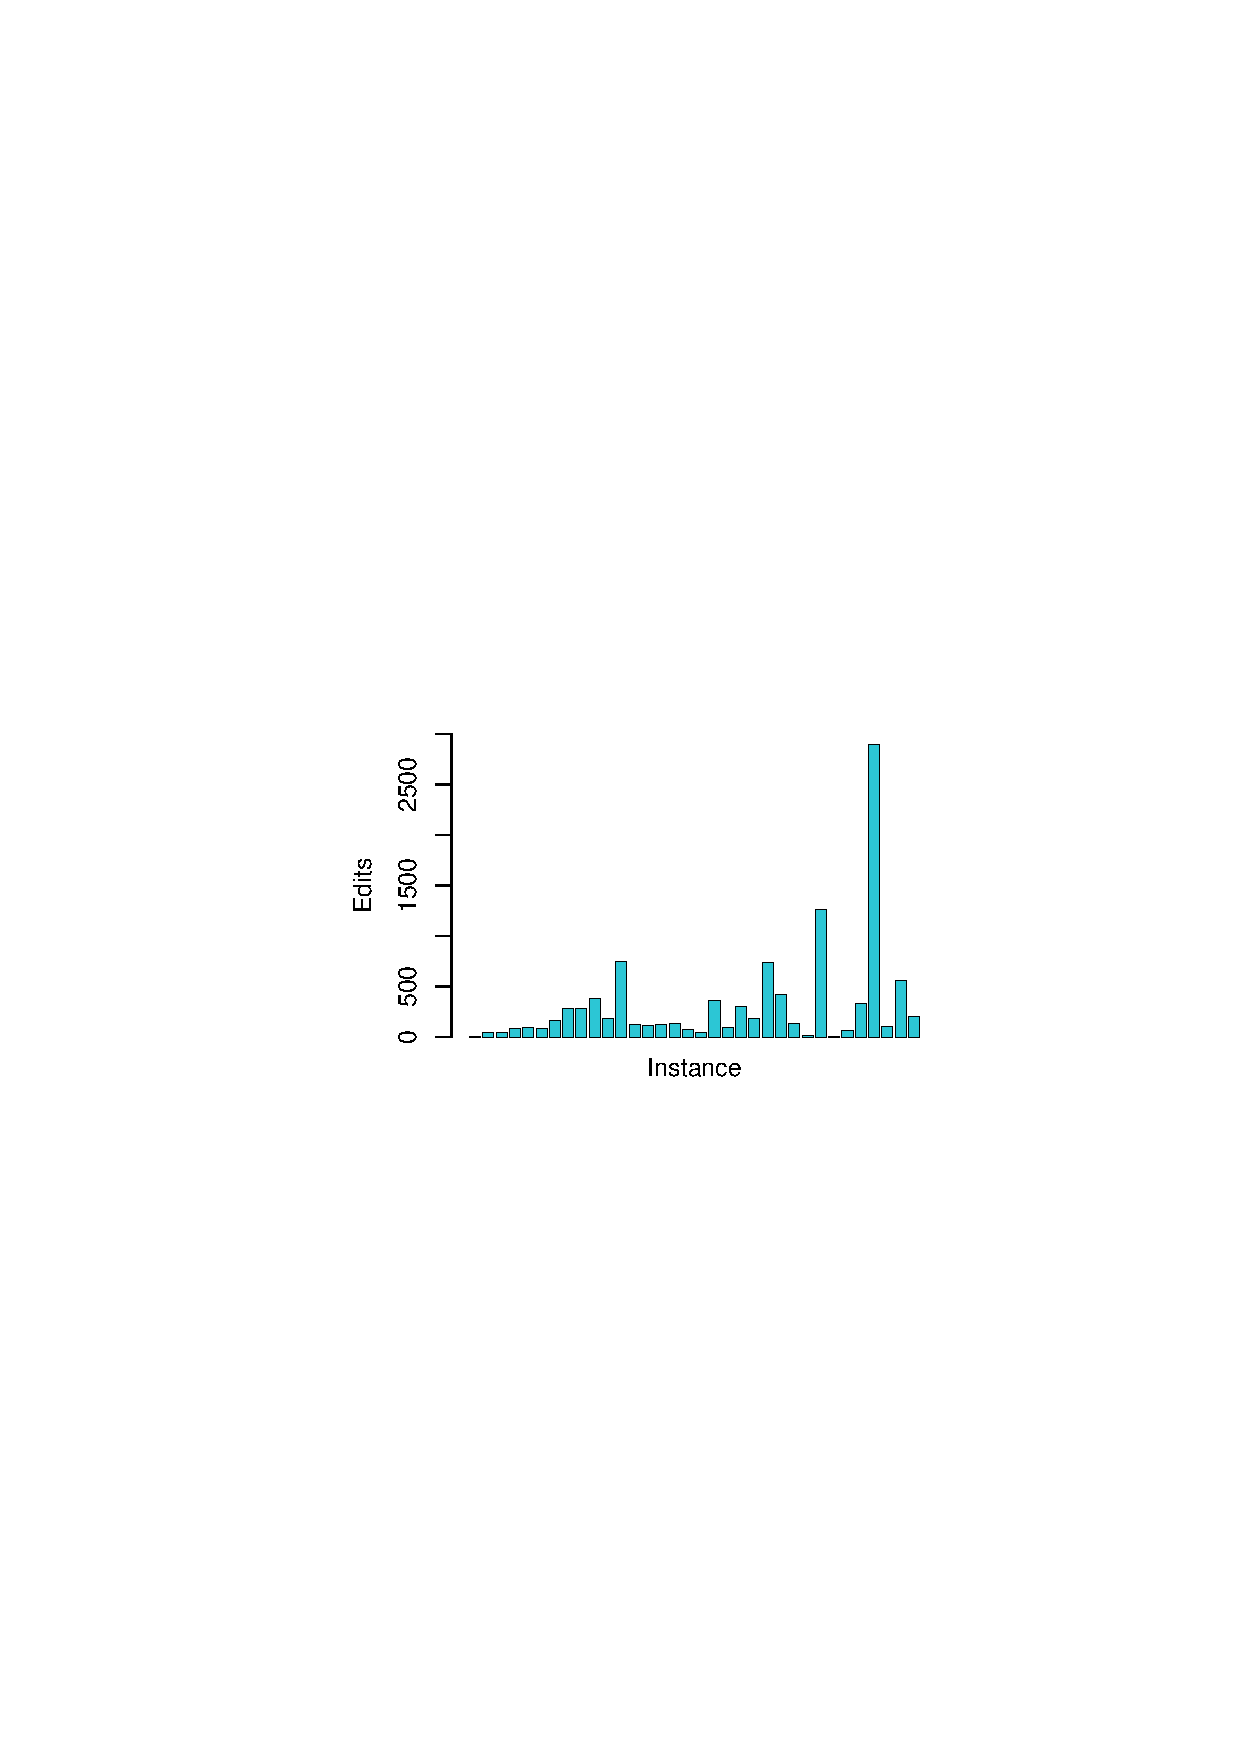
\includegraphics[width=1.0\linewidth]{solution_sizes}
			\subcaption{Solution Sizes}
		\end{subfigure}

		\caption{Public Problem Instances of the PACE Challenge}
		\label{fig:instances}
	\end{figure}
\end{frame}

\begin{frame}
	\frametitle{Results}
	\begin{figure}[h]
		\begin{subfigure}{0.49\textwidth}
			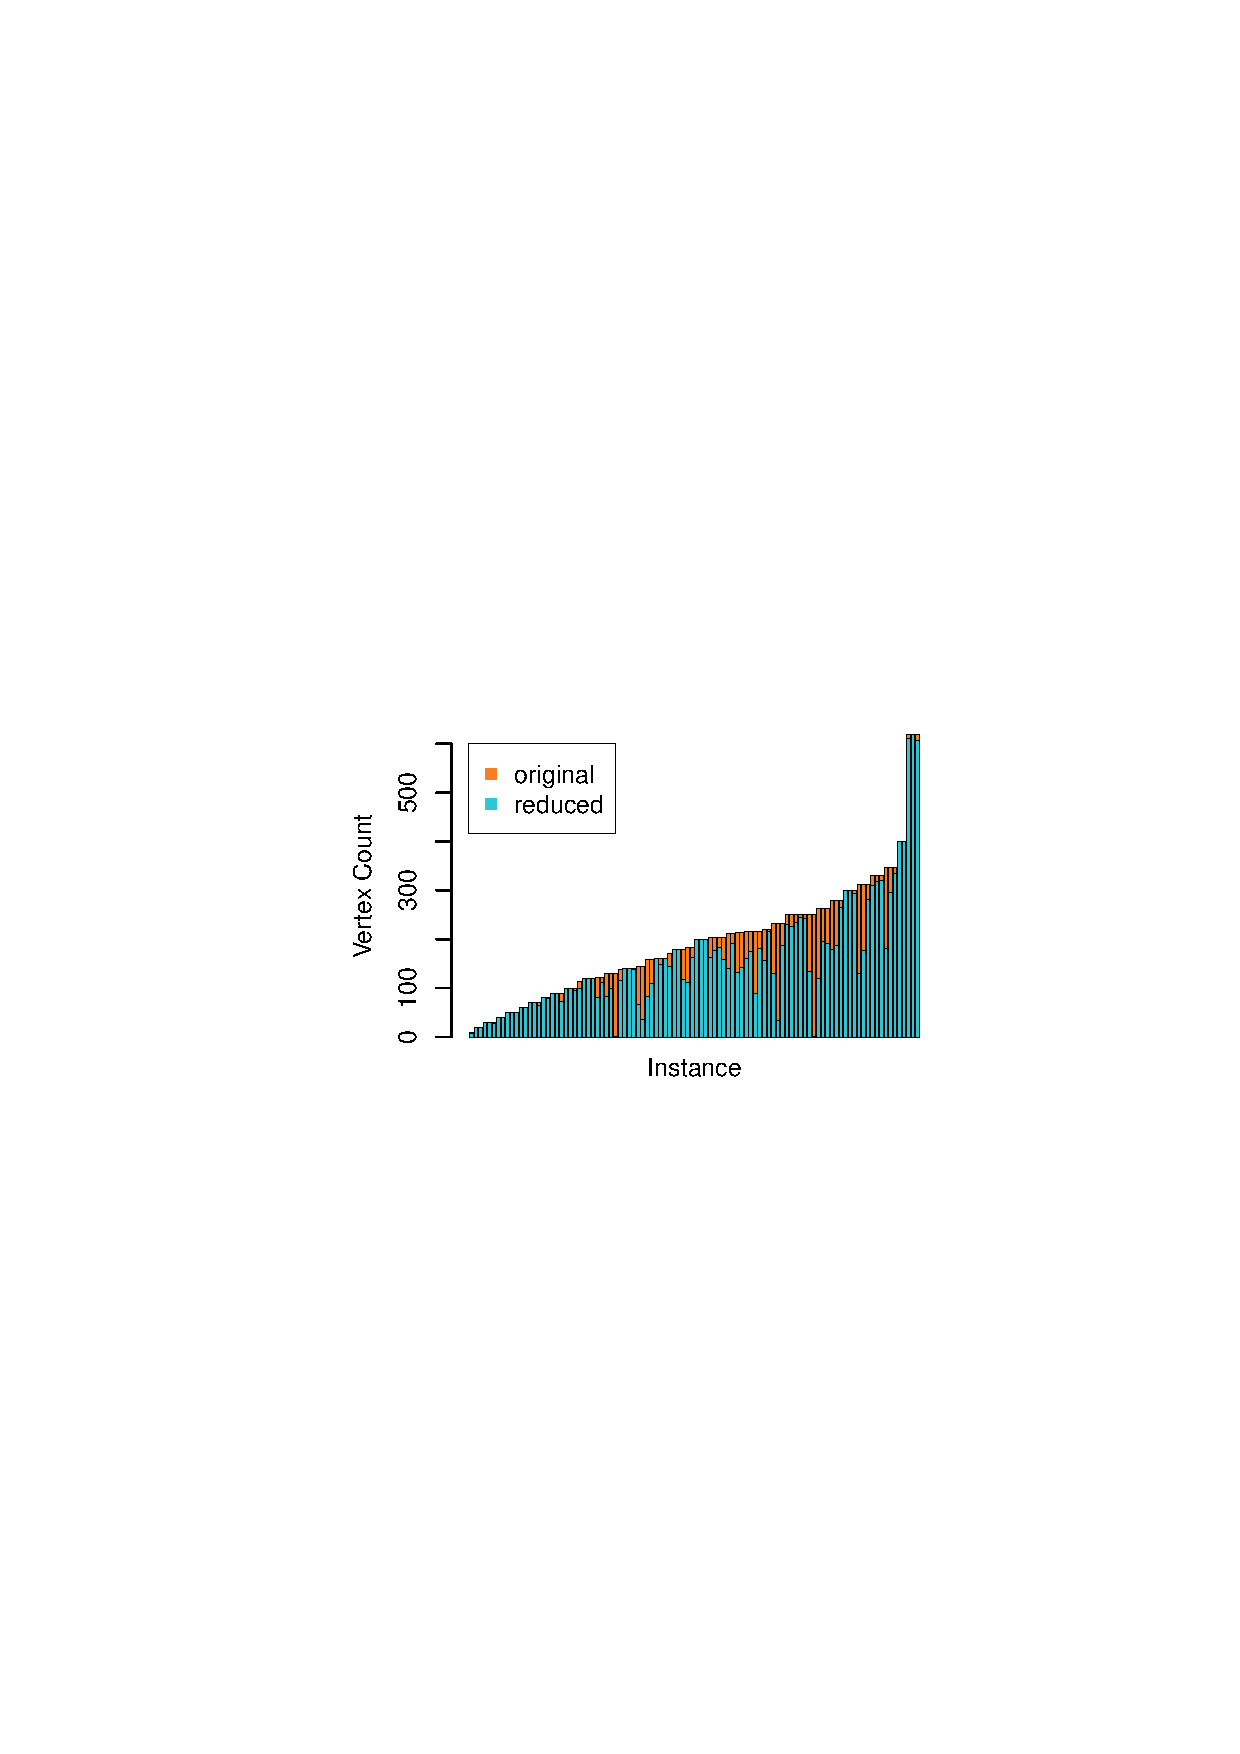
\includegraphics[width=1.0\linewidth]{full_initial_absolute}
		\end{subfigure}
		\begin{subfigure}{0.49\textwidth}
			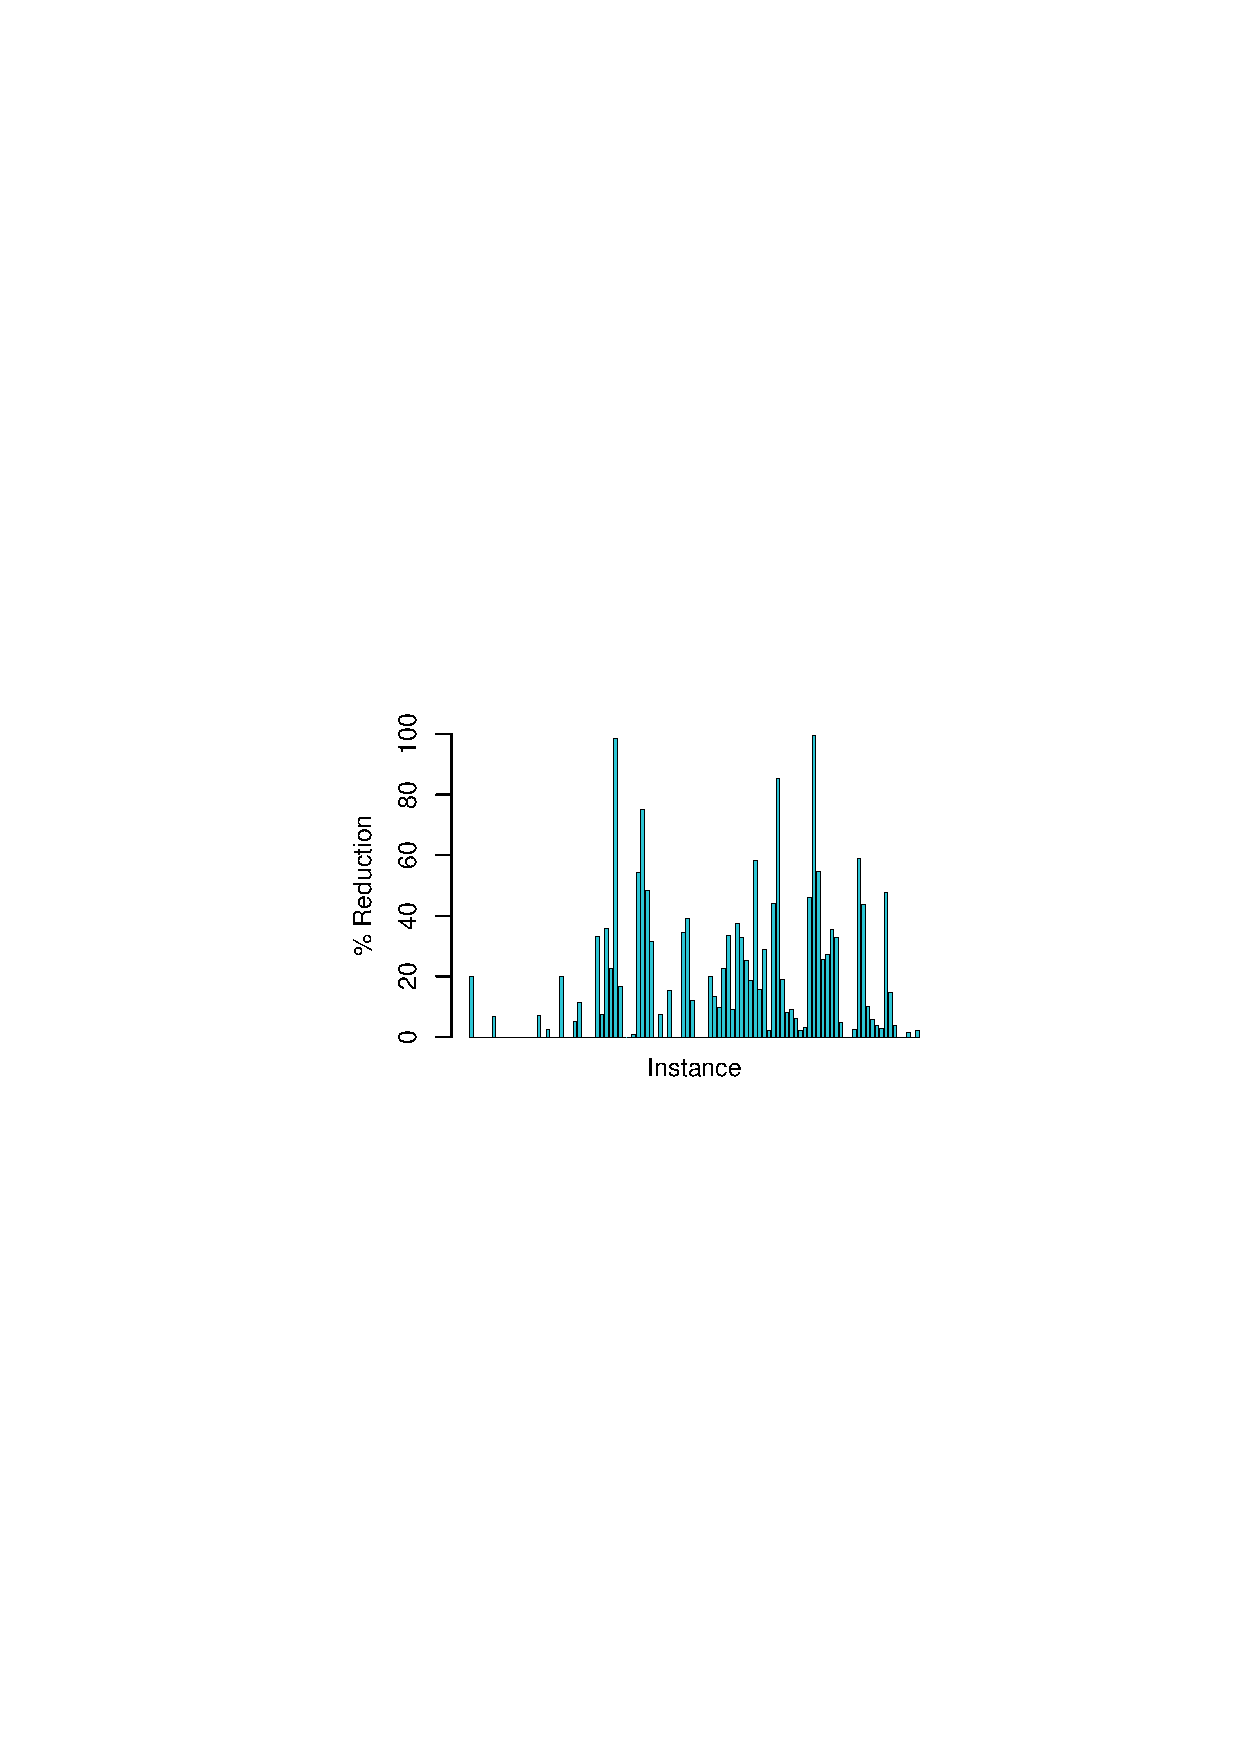
\includegraphics[width=1.0\linewidth]{full_initial_percent}
		\end{subfigure}
		\caption{Full Initial Reduction Effectiveness}
		\label{fig:initial eff}
	\end{figure}
\end{frame}

\begin{frame}
	\frametitle{Outlook \& Conclusion}
	\begin{itemize}
		\item Some additional work done after submission of the thesis, but results still similar
		\item Still a lot of potential: Improved branching strategies exist, and many other
			reduction techniques have been introduced
		\item Solver could also be parallelized relatively easy
		\item Submission to PACE done, results expected in July
	\end{itemize}
\end{frame}

\end{document}
